\chapter[SCP-111]{
    SCP-111 Dragon-Snails™\\
    SCP-111 龙蜗牛™
}

\label{chap:SCP-111}

\begin{figure}[H]
    \centering
    \captionsetup{justification=centering}
    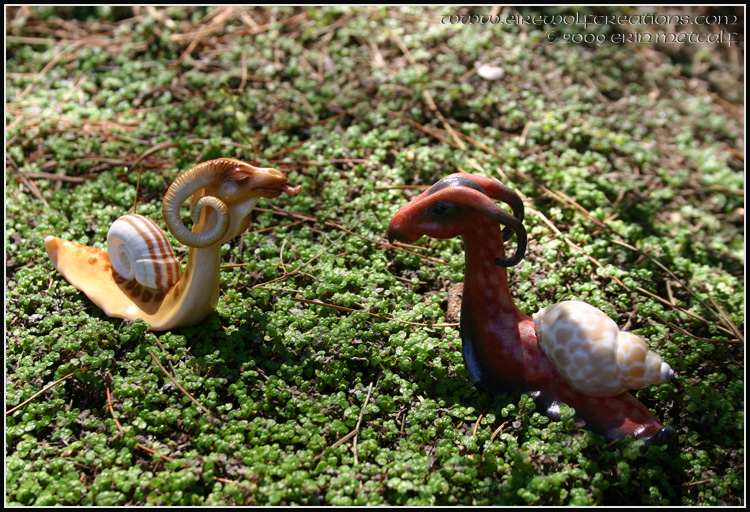
\includegraphics[width=0.5\linewidth]{images/SCP.111.jpg}
    \caption*{2只111的样本,一只“软泥龙”(左侧)和一只“软腹”(右侧),在收容间之中。\\相片由 \href{http://eirewolfcreations.deviantart.com/}{特工 Erin Metcalf} 拍摄}
\end{figure}

\bb{项目编号:}SCP-111

\bb{项目等级:}Safe

\bb{特殊收容措施:}所有被收容的SCP-111样本都应该被收容于19号站点的██████████翼楼之中,在5m x 5m x 5m的一个树脂玻璃房间里,该盒子之中有着一片从其原环境之中移植过来的温和树林环境。栖息地温度将会被保持在30℃。111将由人员进行一周一次的喂食,通过将3kg的冰冻的莴苣(植物学名\ii{Lactuca sativa})放入收容房间之中进行。水将会通过一个自动喷雾系统来给予,该系统会将环境湿度维持在50\%,这既是为了给111供水也是为了防火。在111的繁殖事件之中,人员必须收集所有的蛋并且将它们转送到生物研究翼楼之中进行冷冻。

\bb{描述:}SCP-111是一种很明显是人为制造的类似于蜗牛的无脊椎动物。成年的111样本大约长20cm,宽12cm,高15cm,虽然每一只生物之间的精确尺寸有细微的差别。111和其它蜗牛的不同点在于它有着温血的新陈代谢、复眼、还有由软骨构成的脊柱线状的小“犄角”,并且很明显有着更高的智慧(人员将会被要求阅读测试文档██████作为一个例子),并且有着像脊椎动物一样的复杂的下颚系统;并且,这些物种下的蛋有着硬化的外壳。

最为异常的是,111在其下颚下部有着空囊,里面储存着作为消化过程的副产物的甲烷。一系列{[}数据删除]沿着其内部的气管作为了一个“打火机”的点火装置在这个物种呼吸的时候点燃了这些甲烷,从它们的口中吐出一小股火焰。被称为“火焰喷吐”的事情通常会发生在他们感到压力或者是生气的时候,虽然这并不像是一种主动的破坏行为而更像是一种警告。可以推断出因为那甲烷袋有限制的大小,它限制了111一次能够进行喷火的量,并且这要求很长时间和充足的食物来进行补充。

111的行为也和其他的普通蜗牛不一致,包括吹出或者是吼出很容易就能被人类听到的声音,高等智能在这些测试例如{[}数据删除]之中得到了体现,并且还有双亲抚养他们的后代也体现了这一点。幼体已经被观察到能够铭记它们的双亲、其他同种的特体或者是研究员。基于文档111-a这被认为是一种值得深思的特质,因为这意味着幼体根据拥有者进行不同的铭记\footnote{译注:这里的“铭记”指的是在胚胎时期就开始有记忆的现象,具体请参见各种奇幻小说之中的龙族}。

\bb{历史:}在██\slash ██\slash ████一个有着12颗111的蛋和文档111-a的包裹被邮寄到了{[}数据删除],一个基金会的前台组织。机动特遣队Alpha-4已经确认不能确定以上所述包裹的寄送地点。

\bb{文档111-a:}

\begin{scpbox}

Dr. Wondertainment的新产品,\bb{龙蜗牛™(DRAGON-SNAILS™)}!

给喜欢幻想的孩子的最完美宠物。

照管和孵化指南:

1. 读了这个指南,就轻轻地把蛋从盒子里拿出来,龙蜗牛™的蛋是很容易碎掉的!\\
2. 将蛋放在一个温暖的、安全的地方,然后等上7-10天。\\
3. 拿起你新孵化的龙蜗牛™来让它们好好看看你,让它们认为你就是它们的妈咪。\\
4. 从你的新宠物龙蜗牛™上获得乐趣吧!

要想喂食你的龙蜗牛™,给你的新朋友一点成熟的蔬菜吧:莴苣、球芽甘蓝、豆子、任何你不想要的沙拉配菜!记住给它们喝水,一天一杯。

为了让你更好地享受乐趣,龙蜗牛™有6个种类!让它们繁殖来获得特殊的宠物吧!

\bb{类型:}

1. \bb{软腹®(Slimybellies®):}可爱而又黏糊糊的小伙伴!有着出色的消防车般的红皮肤,小小的黑犄角和肚子,还有有斑点的褐壳!漂亮的知更鸟蛋般蓝色的蛋!

2. \bb{软泥龙®(Oozedrakes®):}好奇的小东西,有着干净的香蕉黄皮肤,卷曲的犄角和条纹壳,淡褐色的壳,就像是小鸡一样!

3. \bb{黏飞龙®(Goowyverns®):}暗蓝灰色的皮肤,较平的壳,并且头上的不平的犄角让黏飞龙®看起来就像是一只小海怪!蛋是梦幻般的玻璃绿色!

4. \bb{团团虫®(Blobworms®):}绿色和金色的条纹,尖尖的壳,和一只独角,更不用提毛茸茸的尾巴了,这些都让团团虫®变成了美妙的宠物!蛋是扁平的,并且有银色的色彩!

5. \bb{辉光龙®(Glowdrakes®):}Dr. Wondertainment的新产品,这些小伙伴看起来就像是蓝黑色的软腹®……直到他们亮起来!那就对了!辉光龙®能够在黑暗之中发光!蛋是金色的还有红色的斑点!

6. \bb{泥飞龙®(Gunkwyverns®):}胖丰满,绿色皮肤,原状的壳,泥飞龙®就是美妙的宠物!蛋是透明的,所以你能够看到小小的龙蜗牛®在里面!

\bb{家长须知:}因为Dr. Wondertainment的龙蜗牛™会喷火,它们已知会导致家庭火灾,为了最大化你的安全和玩乐时间,推荐手持灭火器。尽管如此,Dr. Wondertainment对于一切由于不安全使用龙蜗牛™或是其他产品的做法而导致的受伤、死亡或者是财产损失事件在法律上、道德上或者是经济上都不负责。

在阅读了这个指南并且孵化了龙蜗牛™蛋之后,你就已经同意了以上所说的所有条款并且丧失了诉讼、组织抵制、抗议或者是光荣决斗等等的权利。

好好享受你的买到的产品吧!

\end{scpbox}
